% !TeX root = probability.tex

%%%%%%%%%%%%%%%%%%%%%%%%%%%%%%%%%%%%%%%%%%%%%%%%%%%%%%%%%%%%%

\section{קיץ תשע"ד מועד ב}

\begin{center}
\selectlanguage{english}
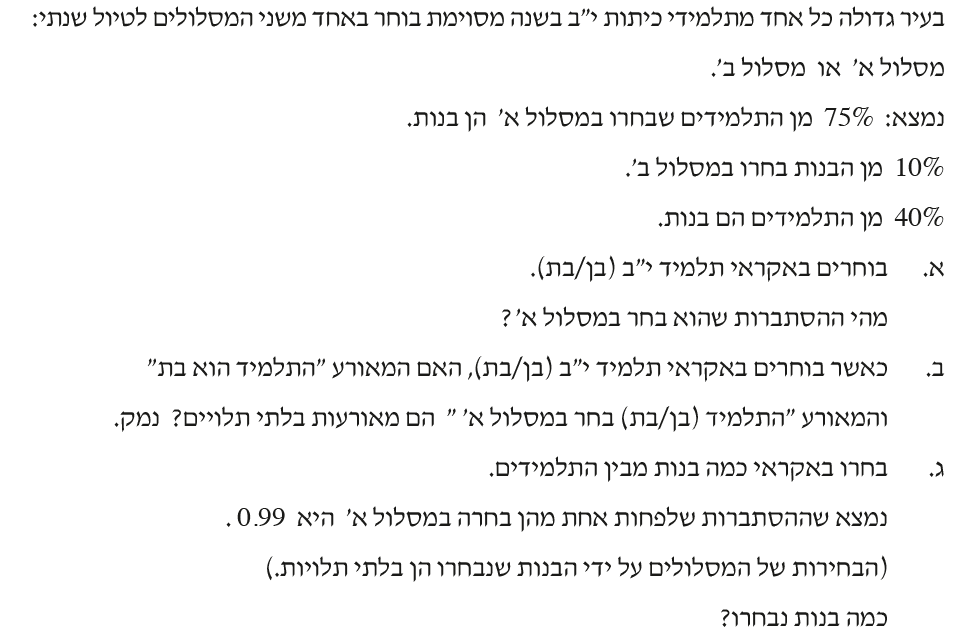
\includegraphics[width=.95\textwidth]{summer-2014b-3}
\end{center}

נמסן את הקבוצות בשאלה:
$G$ \L{(girl)}, $B$ \L{(boy)},
$MA$ \L{(maslul aleph)}, $MB$ \L{(maslul bet)}.
בגלל שיש שני זוגות של קבוצות נציג את ההסתברויות בטבלה. את הטבלה נמלא בשתי דרכים שונות, תחילה ישירות מהנתונים ואחר כך תוך שימוש בהסתברות מותנית.
\begin{center}
\selectlanguage{english}
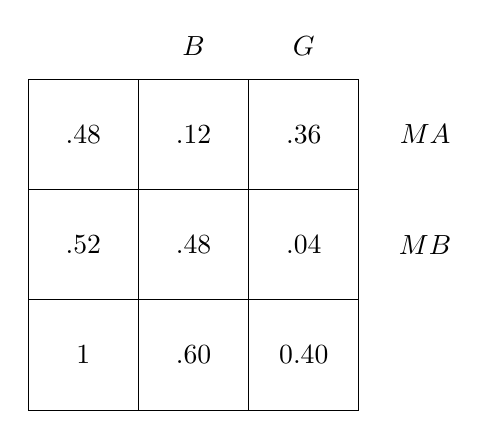
\begin{tikzpicture}[scale=1.4]
\draw (0,0) grid (3,3);
\node at (2.5,3.3) {$G$};
\node at (1.5,3.3) {$B$};
\node at (3.6,2.5) {$MA$};
\node at (3.6,1.5) {$MB$};
%\node at (2.5,2.7) {$.4-.04=$};
\node at (2.5,2.5) {$.36$};
%\node at (0.5,2.7) {$.36/.75=$};
\node at (0.5,2.5) {$.48$};
%\node at (1.5,2.7) {$.48-.36=$};
\node at (1.5,2.5) {$.12$};
%\node at (0.5,1.7) {$1-.48=$};
\node at (0.5,1.5) {$.52$};
\node at (0.5,0.5) {$1$};
%\node at (1.5,0.7) {$1-.4=$};
\node at (1.5,0.5) {$.60$};
%\node at (2.5,0.7) {\bfseries \R{נתון}};
\node at (2.5,0.5) {$0.40$};
%\node at (1.5,1.7) {$.52-.04=$};
\node at (1.5,1.5) {$.48$};
%\node at (2.5,1.7) {$.1\times .4=$};
\node at (2.5,1.5) {$.04$};
\end{tikzpicture}
\end{center}

\textbf{דרך א'}

נתון ש-% 
$P(G)=0.40$
ונתון ש-%
$10\%$
מהם בחרו במסלול ב', ולכן 
$P(G\cap MB)= .04$,
ומהסתברות משלימה
$P(G\cap MA)= .36$.
הנתון האחרון הוא ש-%
$0.75 P(MA) = 0.36$
ולכן 
$P(MA)=0.36/0.75=0.48$.
את שאר התאים ניתן למלא מהסתברויות משלימות.

\textbf{דרך ב'}

שוב נמלא את התא הימני למטה ב-%
$P(G)=0.40$.
נמשיך:
\begin{eqnarray*}
P(MB/G) &=& \frac{P(MB \:\cap\: G)}{P(G)}=0.10\\
P(MB \:\cap\: G) &=& P(G)P(MB/G) = 0.40\cdot 0.10 = 0.04\,.
\end{eqnarray*}
עוד הסתברות מותנית:
\begin{eqnarray*}
P(G/MA) &=& \frac{P(G \:\cap\: MA)}{P(MA)}=0.75\\
P(MA) &=& \frac{P(G \:\cap\: MA)}{P(G/MA)}=\frac{0.36}{0.75}=0.48\,,
\end{eqnarray*}
ונמלא את שאר התאים באמצעות הסתברויות משלימות.

\textbf{סעיף א}

$P(MA)=0.48$.

\textbf{סעיף ב}
\begin{eqnarray*}
P(G\cap MA) &=&0.36\\
P(G)P(MA)&=&0.40\cdot 0.48=0.19\,.
\end{eqnarray*}
$0.36\neq 0.19$
ולכן המאורעות אינם בלתי תלויים.

\textbf{סעיף ג}

ניתן לחשב "לפחות אחת" על ידי חישוב הסתברות של "אף אחת". ההסתברות שבת לא תבחר מסלול א' היא ההסתברות שהיא תבחר מסלול ב':
\begin{eqnarray*}
P(MB/G) &=& \frac{P(MB \:\cap\: G}{P(G)}= \frac{0.04}{0.40}=0.10\\
(0.10)^n&=&1-0.99=0.01\\
n&=&2\,.
\end{eqnarray*}

%%%%%%%%%%%%%%%%%%%%%%%%%%%%%%%%%%%%%%%%%%%%%%%%%%%%%%%%%%%%%%%%%%%

\section{קיץ תשע"ד מועד א}

\begin{center}
\selectlanguage{english}
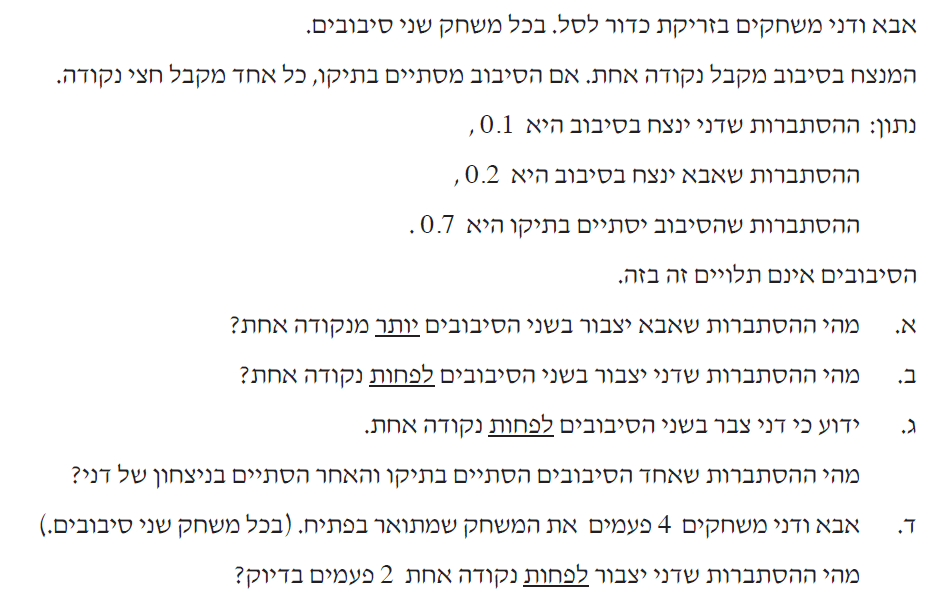
\includegraphics[width=.9\textwidth]{summer-2014a-3}
\end{center}

נסמן ב-%
$D1, D2$ \L{(dani)}
את המאורע שדני מנצח בסיבוב אחד או שניים, נסמן ב-%
$A1, A2$ \L{(abba)}
את המאורע שאבא מנצח בסיבוב אחד או שניים, ונסמן ב-%
$T1, T2$ \L{(teku)}
את המאורע שיהיה תיקו בסיבוב אחד או שניים. השאלה שואלת על סדרה של שני סבבים וזה מכוון לעץ הסתברויות (בעמוד הבא). בסוף כל מסלול רשום מספר הנקודות שאבא צבר ומספר הנקודות שדני צבר.

\begin{figure}
\begin{center}
\selectlanguage{english}
\begin{tikzpicture}
[align=left,grow=right,
level 1/.append style={level distance=3cm,sibling distance=9em},
level 2/.append style={level distance=4cm,
                       sibling distance=3.5em}]
\node[left] {$0$} % root
child {
  node[right] {$\frac{1}{2}$}
    child {
      node[below right,xshift=10pt,yshift=4pt] {$(i) A2=1,D2=1$}
      edge from parent node[below,yshift=-1mm] {$0.7$}
    }
    child {
      node[right,xshift=10pt] 
        {$(h) A2=\frac{1}{2},D2=\frac{1}{2}$}
      edge from parent node[below,xshift=4mm] {$0.1$}
    }
    child {
      node[right,xshift=10pt] 
        {$(g) A2=1\frac{1}{2},D2=\frac{1}{2}$}
      edge from parent node[above,yshift=1mm] {$0.2$}
    }
    edge from parent 
      node[below,xshift=-4mm,yshift=-3mm] {\R{תיקו} $0.7$}
}
child {
  node[right] {$0$}
    child {
      node[right,xshift=10pt] 
        {$(f) A2=\frac{1}{2},D2=1\frac{1}{2}$}
      edge from parent node[below,yshift=-1mm] {$0.7$}
    }
    child {
      node[right,xshift=10pt] {$(e) A2=0,D2=2$}
      edge from parent node[below,xshift=4mm] {$0.1$}
    }
    child {
      node[right,xshift=10pt] {$(d) A2=1,D2=1$}
      edge from parent node[above,yshift=1mm] {$0.2$}
    }
    edge from parent 
      node[below] {\R{דני} $0.1$}
}
child {
  node[right] {$1$}
    child {
      node[right,xshift=10pt] {$(c) A2=1\frac{1}{2},D2=\frac{1}{2}$}
      edge from parent node[below,yshift=-1mm] {$0.7$}
    }
    child {
      node[right,xshift=10pt] {$(b) A2=1,D2=1$}
      edge from parent node[below,xshift=4mm] {$0.1$}
    }
    child {
      node[above right,xshift=10pt] {$(a) A2=2, D2=0$}
      edge from parent node[above,yshift=1mm] {$0.2$}
    }
    edge from parent
       node[above,xshift=-4mm,yshift=3mm] {\R{אבא} $0.2$}
};
\end{tikzpicture}
\end{center}
\end{figure}

\textbf{סעיף א}

במסלול בהם אבא צובר יותר מנקודה אחת הם
\L{(a), (c), (g)},
וההסתברות היא:
\[
P(A2>1)=0.2\cdot 0.2 \,+\, 0.2\cdot 0.7 \,+\, 0.7\cdot 0.2 \,=\,0.32\,.
\]


\textbf{סעיף ב}

המסלולים בהם דני צבר לפחות נקודה אחת הם
\L{(b), (d), (e), (f), (h), (i)}
וההסתברות היא:
\[
P(D2\geq 1)=0.2\cdot 0.1 \,+\,0.1\cdot 0.2 \,+\, 0.1\cdot 0.1 \,+\,0.1\cdot 0.7 \,+\, 0.7\cdot 0.1\,+\,0.7\cdot 0.7\,=\,0.68\,.
\]


\textbf{סעיף ג}

הניסוח "ידוע" מכוון להסתברות מותנית, אבל
$D1\cup T1\subseteq D2\geq 1$
ולכן:
\begin{eqnarray*}
P((D1\cup T1)/D2\geq 1)&=&\frac{P((D1\cup T1) \:\cap\: D2\geq 1)}
  {D2\geq 1}\\
  &=&\frac{P(D1\cup T1)}{D2\geq 1}\\
\frac{0.1\cdot 0.7 \,+\, 0.7\cdot 0.1}{0.68} &=& \frac{7}{34}= 0.2059\,,  
\end{eqnarray*}
כי המסלולים המתאימים הם 
\L{(f), (h)}.

\textbf{סעיף ד}

נשמתמש בנוסחת ברנולי כי למצוא את ההסתברות לבדיוק פעמיים:
\[
{4\choose 2}P(D2)^2\: (1-P(D2)^2 =
{4\choose 2} (0.32)^2 (0.68)^2= 0.2841\,.
\]

%%%%%%%%%%%%%%%%%%%%%%%%%%%%%%%%%%%%%%%%%%%%%%%%%%%%%%%%

\section{חורף תשע"ד}

\begin{center}
\selectlanguage{english}
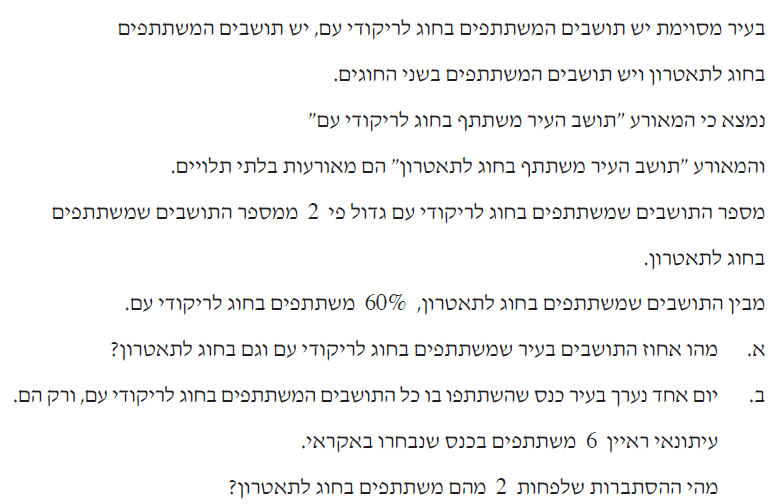
\includegraphics[width=.9\textwidth]{winter-2014-3}
\end{center}

נסמן ב-%
$T$ \L{(theatron)}
את המשתתפים בתאטרון ונסמן ב-%
$R$ \L{(rikudei)}
את המשתתפים בריקודי עם. המילה "מבין" מכוונת להתסברות מותנית. ההסתברויות הן של זוגות של מאורעות ולכן נשתמש בטבלה.


נתון
$P(R/T)=0.6$
ושהאירועים בלתי תלויים. נחשב:
\[
P(R/T)=\frac{P(R\cap T)}{P(T)}=\frac{P(R)\cdot P(T)}{P(T)}=P(R)=0.06\,.
\]
ביחד עם הנתון
$P(R)=2P(T)$
נתחיל למלא את הטבלה:
\begin{center}
\selectlanguage{english}
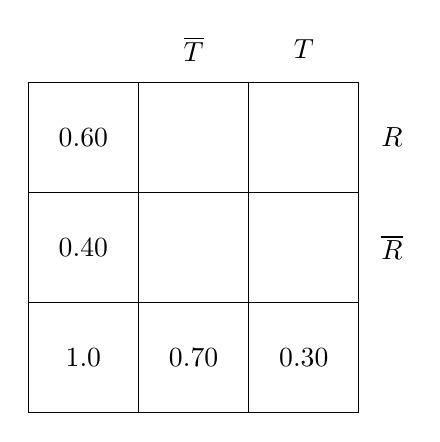
\begin{tikzpicture}[scale=1.4]
\draw (0,0) grid (3,3);
\node at (2.5,3.3) {$T$};
\node at (1.5,3.3) {$\overline{T}$};
\node at (3.3,2.5) {$R$};
\node at (3.3,1.5) {$\overline{R}$};
\node at (0.5,2.5) {$0.60$};
\node at (2.5,0.5) {$0.30$};
\node at (.5,.5) {$1.0$};
\node at (1.5,.5) {$0.70$};
\node at (.5,1.5) {$0.40$};
\end{tikzpicture}
\end{center}
שוב נסתמך על העובדה שהאירועים בלתי תלויים ונקבל:
\[
P(R\cap T)=P(R)\cdot P(T)=0.60\cdot 0.30=0.18\,,
\]
וניתן למלא את הטבלה לפי הסתברויות משלימות:
\begin{center}
\selectlanguage{english}
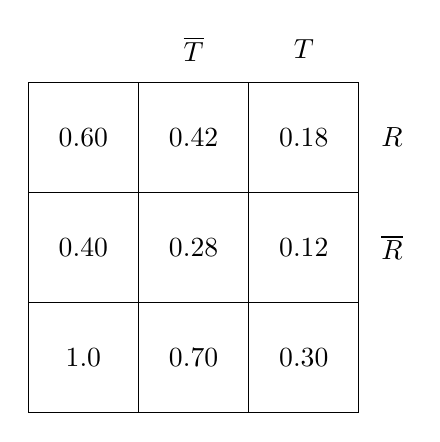
\begin{tikzpicture}[scale=1.4]
\draw (0,0) grid (3,3);
\node at (2.5,3.3) {$T$};
\node at (1.5,3.3) {$\overline{T}$};
\node at (3.3,2.5) {$R$};
\node at (3.3,1.5) {$\overline{R}$};
\node at (2.5,2.5) {$0.18$};
\node at (0.5,2.5) {$0.60$};
\node at (1.5,2.5) {$0.42$};
\node at (0.5,1.5) {$0.40$};
\node at (0.5,0.5) {$1.0$};
\node at (1.5,0.5) {$0.70$};
\node at (2.5,0.5) {$0.30$};
\node at (1.5,1.5) {$0.28$};
\node at (2.5,1.5) {$0.12$};
\end{tikzpicture}
\end{center}

\textbf{סעיף א}

$P(R\cap T)=0.18$.

\textbf{סעיף ב}

הניסוח "כל התושבים המשתתפים בחוג לריקודי עם, ורק הם" מכוונות להסתברות מותנית:
\[
P(T/R) = \frac{P(T\cap R)}{P(R)} = \frac{P(T)P(R)}{P(R)}= P(T)=0.30\,.
\]
כדי לחשב "לפחות שניים" נשתמש בנוסחת ברנולי ונחשב את המשלים ל-"אפס או אחד":
\[
P(T\geq 2/R)=1-{6\choose 0}(0.3)^0(0.7)^6 -{6\choose 1}(0.3)^1(0.7)^5=0.5798\,.
\]
